\section{Results}\label{sec:results}
To test the performance of the proposed algorithms, each was tested on several maps. Each solver was run 5 times in identical environments, keeping track of the time it took to solve the map, as well as the number of steps proposed in the solution. Since not all solvers were able to find a solution within a time limit of 60 seconds, only results for four solvers are given: BestFS, Genetic Algorithm, Iterative Deepening Search and Iterative Deepening A*. The maps are denoted Map 1, in figure \ref{fig:map1}, and Map 2, in figure \ref{fig:map2}.

\begin{figure}
\center
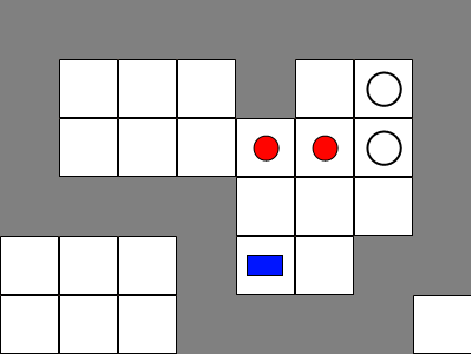
\includegraphics[width=\columnwidth]{./images/map_1.png}
\caption{Map 1}
\label{fig:map1}
\end{figure}

\begin{figure}
\center
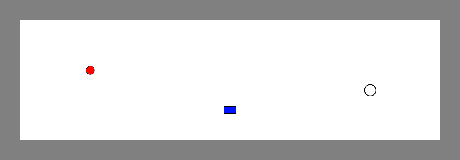
\includegraphics[width=\columnwidth]{./images/map_2.png}
\caption{Map 2}
\label{fig:map2}
\end{figure}

The results for the given algorithms are listed in figure \ref{fig:result1}. Error bars indicate a 95\% confidence interval after 5 repeated tests of each algorithm for each map. 

\begin{figure*}
\center
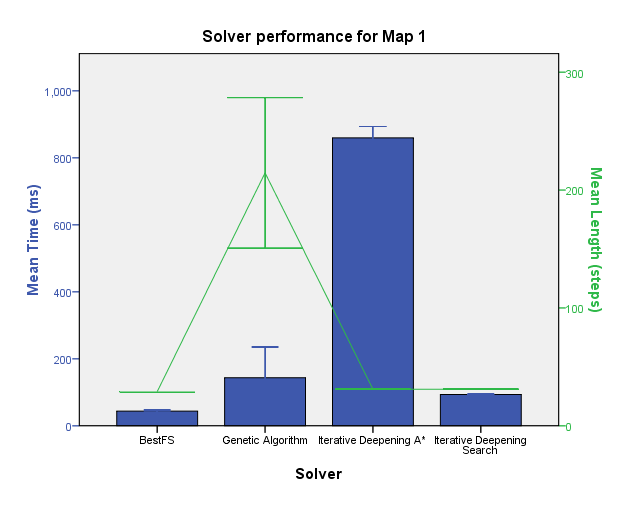
\includegraphics[width=\columnwidth]{./images/performance_map27.png}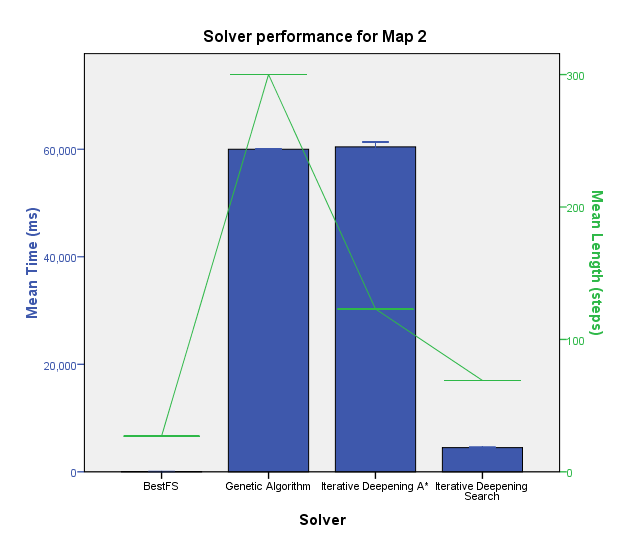
\includegraphics[width=\columnwidth]{./images/performance_map28.png}
\caption{Results Map 1 and Map 2}
\label{fig:result1}
\end{figure*}


\subsection{Performance on Map 1}
It should be clear from the performance on Map 1 in figure \ref{fig:result1} that a great deviation exists between solvers, both in their proposed solutions as well as the time they require to obtain those solutions. In general, BestFS performs best here, as it finds an efficient solution fast, compared to the other algorithms. Interesting to note is the great deviation in solution length, found by the Genetic Algorithm solver: as is to be expected, the randomness of this approach creates great variation, and longer individuals are more likely to solve the problem.

Interestingly enough, Iterative Deepening A* performs worst of all four solvers. There is no easy explanation for this: the solution it finds appears to be close to optimal, yet it is very slow. This hints at an inefficiency in the algorithm that might be resolved in the future.

\subsection{Performance on Map 2}
A similar result can be seen for Map 2: BestFS again performs fast, and finds the shortest solution. Iterative Deepening Search is comparatively close, while the Iterative Deepening A* algorithm reaches the 60 second time limit. The Genetic Algorithm does in fact reach that limit and did not find a solution on any trial. Likewise, its proposed solution length is the maximum individual size of 300 steps.

\subsection{General Performance}
From the given data, it should be clear that the solvers may all be capable of solving simple maps, yet are not equally effective at doing so. The BestFS algorithm performs well under any circumstance, though performance of the Genetic Algorithm solver varies greatly. IDA* performance is an order of magnitude worse than BestFS performance, even though both algorithms share many common assumptions: this can be cause for further investigation. Surprisingly enough, the generic Iterative Deepening Search algorithm keeps performing adequately in these maps, even though it is an uninformed search method.

The algorithms are also tested on additional maps. However, only BestFS was capable of solving more complex maps within the given time limit. General observations from these results indicate that solution length and time requirement are correlated; however, as the solution length for Map 2 is lower than the solution length for Map 1, yet the time requirement is greater, it is quite likely that this correlation will prove to be a complex one.




